\documentclass[11pt]{amsart}
\usepackage{geometry}                % See geometry.pdf to learn the layout options. There are lots.
\geometry{a4paper}                   % ... or a4paper or a5paper or ... 
%\geometry{landscape}                % Activate for for rotated page geometry
%\usepackage[parfill]{parskip}    % Activate to begin paragraphs with an empty line rather than an indent
\usepackage{graphicx}
\usepackage{amssymb}
\usepackage{epstopdf}
\usepackage{listings}

\DeclareGraphicsRule{.tif}{png}{.png}{`convert #1 `dirname #1`/`basename #1 .tif`.png}

\title{Experimenting Summations with OpenMP}
\author{Minqi Pan}
%\date{}                                           % Activate to display a given date or no date

\begin{document}
\maketitle

\section{Overview}
The result was obtained by calculating $\sum_{i=1}^{4294967296}i=9223372034707292160$ using $1,2,\dots,10$ threads on a Intel(R) Core(TM) i7-7820HQ 2.90GHz CPU which has $4$ physical cores and $8$ logical cores.

\begin{figure}[ht]
\begin{center}
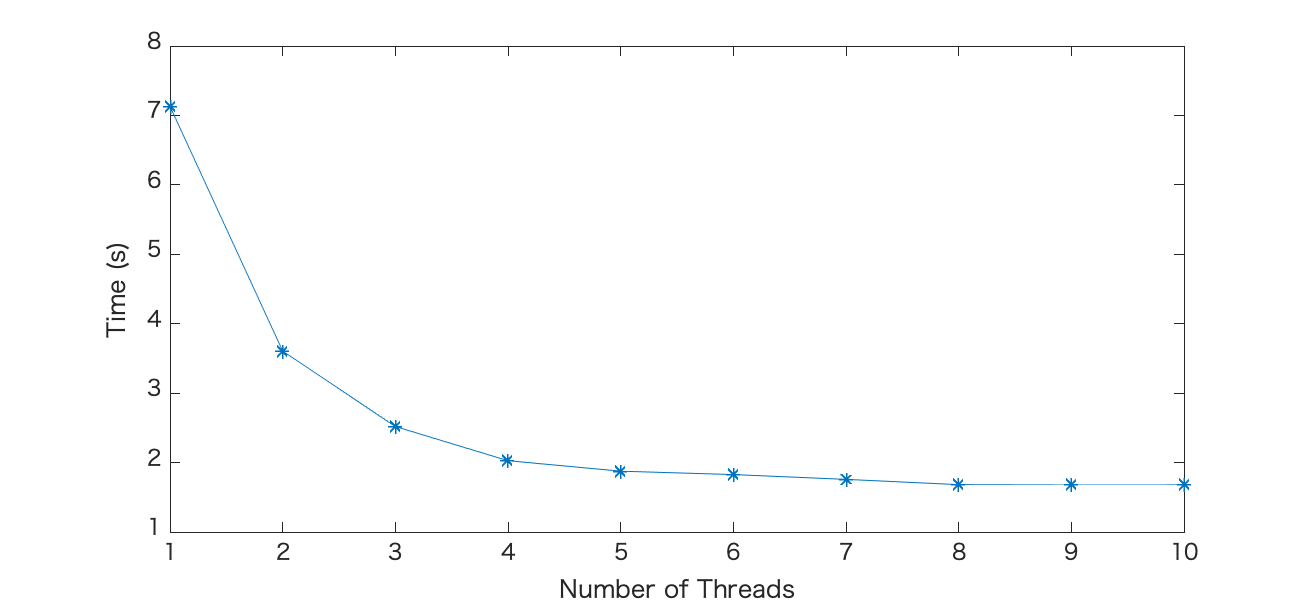
\includegraphics[width=.8\textwidth]{experimenting_summations_with_openmp.png}
\end{center}
\end{figure}

\section{Result}

\[
\begin{bmatrix}
1&2&3&4&5&6&7&8&9&10\\
7.131&3.606&2.519&2.027&1.876&1.827&1.758&1.682&1.677&1.678
\end{bmatrix}
\]


\section{Code}

\renewcommand{\ttdefault}{pcr}
\lstinputlisting[language=c++,basicstyle=\ttfamily,numbers=left,xleftmargin=1cm,frame=L,keepspaces=true]{experimenting_summations_with_openmp.cpp}

\end{document}
